\chapter{System Specification}
\label{ch:specification}

\section{System Requirements}
\label{sec:requirements}

\subsection{Functional Requirements}

The system shall implement the \texttt{rv32im\_zicsr\_zve32x\_zvl128b} instruction set
architecture. The following functional requirements are derived from the RVV
specification \cite{rvv-spec-1-0} and the project objectives stated in
Chapter~\ref{ch:introduction}.

\begin{enumerate}[label=FR-\arabic*.]
  \item The scalar core shall execute all RV32I base instructions and all RV32M
        multiply/divide instructions.
  \item The scalar core shall support CSR access instructions (\texttt{CSRRW},
        \texttt{CSRRS}, \texttt{CSRRC}, and their immediate variants) to read the
        vector length, vector type, and vector length-in-bytes registers.
  \item The \gls{vpu} shall implement all Zve32x integer arithmetic instructions:
        \texttt{vadd}, \texttt{vsub}, \texttt{vrsub}, \texttt{vmul}, \texttt{vmulh},
        \texttt{vmulhu}, \texttt{vmulhsu}, and their widening variants.
  \item The \gls{vpu} shall implement logical instructions: \texttt{vand}, \texttt{vor},
        \texttt{vxor} in VV, VX, and VI encoding variants.
  \item The \gls{vpu} shall implement shift instructions: \texttt{vsll}, \texttt{vsrl},
        \texttt{vsra} in VV, VX, and VI variants.
  \item The \gls{vpu} shall implement integer comparison and mask-generating instructions:
        \texttt{vmseq}, \texttt{vmsne}, \texttt{vmslt}, \texttt{vmsltu}, \texttt{vmsle},
        \texttt{vmsleu}, \texttt{vmsgt}, \texttt{vmsgtu}.
  \item The \gls{vpu} shall implement integer reduction instructions: \texttt{vredsum},
        \texttt{vredmax}, \texttt{vredmin}, \texttt{vredmaxu}, \texttt{vredminu}.
  \item The \gls{vpu} shall implement unit-stride vector load and store instructions:
        \texttt{vle8.v}, \texttt{vle16.v}, \texttt{vle32.v}, \texttt{vse8.v},
        \texttt{vse16.v}, \texttt{vse32.v}.
  \item The \gls{vpu} shall implement integer min/max instructions: \texttt{vmin},
        \texttt{vmax}, \texttt{vminu}, \texttt{vmaxu}.
  \item The \gls{vpu} shall implement \texttt{vmv.v.x} (broadcast scalar to all elements)
        and \texttt{vmv.x.s} (move element 0 to scalar register).
  \item The \gls{vpu} shall implement carry-in arithmetic: \texttt{vadc},
        \texttt{vmadc}.
  \item The \gls{vpu} shall implement vector configuration instructions:
        \texttt{vsetvli}, \texttt{vsetvl}, \texttt{vsetivli}.
  \item The system shall include a UART peripheral at memory address \texttt{0xFF000000}
        supporting 8-N-1 framing at 115200~baud, accessible through MMIO load/store
        instructions.
  \item The system shall support Harvard memory architecture: a read-only 8~KB
        instruction memory at \texttt{0x00000000} and a read/write 64~KB data memory
        at \texttt{0x00000000} in the data address space.
\end{enumerate}

\subsection{Non-Functional Requirements}

\begin{enumerate}[label=NF-\arabic*.]
  \item \textbf{Synthesisability.} All RTL in the \texttt{/rtl/} directory shall be
        synthesisable by Quartus Prime and by standard ASIC synthesis tools (Yosys,
        Synopsys DC). No \texttt{initial} blocks, no \texttt{\$display}/\texttt{\$time}
        tasks, no combinational latches, and no delays (\texttt{\#N}) shall appear in
        any synthesisable file.
  \item \textbf{Synchronous active-low reset.} All registers shall be initialised
        through a synchronous active-low \texttt{rst\_n} signal. No asynchronous reset
        paths shall exist in the production RTL (the FPGA-specific \texttt{d\_ff.sv}
        wrapper is excluded from this requirement).
  \item \textbf{Parameterised widths.} All bus widths that depend on VLEN, SEW, or
        LMUL shall be expressed using \texttt{parameter} or \texttt{localparam}
        declarations. No hardcoded constants that would require manual editing to
        retarget the design.
  \item \textbf{Target clock frequency.} The design shall target a minimum
        $F_\text{max}$ of 50~MHz on the Intel Cyclone~V device
        (DE10-Standard) \cite{de10standard} at typical process, voltage, and temperature
        conditions, enabling real-time processing of at least one image row per
        millisecond at VLEN=128.
  \item \textbf{Verification gate.} A regression testbench of 172 directed tests shall
        achieve 100\% pass rate before any RTL change is considered complete.
  \item \textbf{Code style.} All RTL shall use \texttt{logic} types (not \texttt{wire}/
        \texttt{reg} distinctions), \texttt{always\_ff}/\texttt{always\_comb} blocks
        (not \texttt{always @(*)}), and \texttt{typedef enum} for FSM state types.
\end{enumerate}

\section{ISA Specification}
\label{sec:isa-spec}

\subsection{Instruction Encoding Conventions}

All RVV instructions use the OP-V opcode (\texttt{7'b101\_0111}). The \texttt{funct3}
field selects the operand encoding class (VV, VX, VI, etc.). The \texttt{funct6} field
selects the specific operation within the class. The \texttt{vm} bit (\texttt{inst[25]})
controls masking: \texttt{vm=1} means unmasked (all elements active),
\texttt{vm=0} means masked by \texttt{v0}.

\subsection{Supported Instructions by Category}

Tables~\ref{tab:instr-arith}--\ref{tab:instr-lsu} list all supported instructions
with their opcode, funct3, funct6, and operand type.

\begin{table}[H]
  \centering
  \caption{Arithmetic instructions (OPIVV/OPIVX/OPIVI)}
  \label{tab:instr-arith}
  \begin{tabular}{@{}llllll@{}}
    \toprule
    \textbf{Instruction} & \textbf{funct6} & \textbf{funct3 (VV)} & \textbf{funct3 (VX)} & \textbf{funct3 (VI)} & \textbf{Notes} \\
    \midrule
    \texttt{vadd.vv/vx/vi}   & \texttt{000000} & \texttt{000} & \texttt{100} & \texttt{011} & Signed/unsigned add \\
    \texttt{vsub.vv/vx}      & \texttt{000010} & \texttt{000} & \texttt{100} & ---          & Subtract \\
    \texttt{vrsub.vx/vi}     & \texttt{000011} & ---          & \texttt{100} & \texttt{011} & Reverse subtract \\
    \texttt{vmin.vv/vx}      & \texttt{000101} & \texttt{000} & \texttt{100} & ---          & Signed minimum \\
    \texttt{vminu.vv/vx}     & \texttt{000100} & \texttt{000} & \texttt{100} & ---          & Unsigned minimum \\
    \texttt{vmax.vv/vx}      & \texttt{000111} & \texttt{000} & \texttt{100} & ---          & Signed maximum \\
    \texttt{vmaxu.vv/vx}     & \texttt{000110} & \texttt{000} & \texttt{100} & ---          & Unsigned maximum \\
    \texttt{vadc.vvm/vxm}    & \texttt{010000} & \texttt{000} & \texttt{100} & ---          & Add with carry (\texttt{vm=0}) \\
    \texttt{vmadc.vvm/vxm}   & \texttt{010001} & \texttt{000} & \texttt{100} & ---          & Mask carry out \\
    \bottomrule
  \end{tabular}
\end{table}

\begin{table}[H]
  \centering
  \caption{Logical and shift instructions}
  \label{tab:instr-logic}
  \begin{tabular}{@{}lllll@{}}
    \toprule
    \textbf{Instruction} & \textbf{funct6} & \textbf{funct3 (VV)} & \textbf{funct3 (VX/VI)} & \textbf{Notes} \\
    \midrule
    \texttt{vand.vv/vx/vi}  & \texttt{001001} & \texttt{000} & \texttt{100}/\texttt{011} & Bitwise AND \\
    \texttt{vor.vv/vx/vi}   & \texttt{001010} & \texttt{000} & \texttt{100}/\texttt{011} & Bitwise OR \\
    \texttt{vxor.vv/vx/vi}  & \texttt{001011} & \texttt{000} & \texttt{100}/\texttt{011} & Bitwise XOR \\
    \texttt{vsll.vv/vx/vi}  & \texttt{010101} & \texttt{000} & \texttt{100}/\texttt{011} & Logical left shift \\
    \texttt{vsrl.vv/vx/vi}  & \texttt{010000} & \texttt{000} & \texttt{100}/\texttt{011} & Logical right shift \\
    \texttt{vsra.vv/vx/vi}  & \texttt{010010} & \texttt{000} & \texttt{100}/\texttt{011} & Arithmetic right shift \\
    \bottomrule
  \end{tabular}
\end{table}

\begin{table}[H]
  \centering
  \caption{Multiplication instructions (OPIVV / OPMVV / OPMVX)}
  \label{tab:instr-mul}
  \begin{tabular}{@{}lllll@{}}
    \toprule
    \textbf{Instruction} & \textbf{funct6} & \textbf{funct3 (VV)} & \textbf{funct3 (VX)} & \textbf{Notes} \\
    \midrule
    \texttt{vmul.vv/vx}      & \texttt{100101} & \texttt{010} & \texttt{110} & Low 32 bits of product \\
    \texttt{vmulh.vv/vx}     & \texttt{100111} & \texttt{010} & \texttt{110} & Signed$\times$signed high \\
    \texttt{vmulhu.vv/vx}    & \texttt{100100} & \texttt{010} & \texttt{110} & Unsigned$\times$unsigned high \\
    \texttt{vmulhsu.vv/vx}   & \texttt{100110} & \texttt{010} & \texttt{110} & Signed$\times$unsigned high \\
    \texttt{vwmul.vv/vx}     & \texttt{111011} & \texttt{010} & \texttt{110} & Widening signed$\times$signed \\
    \texttt{vwmulu.vv/vx}    & \texttt{111000} & \texttt{010} & \texttt{110} & Widening unsigned$\times$unsigned \\
    \texttt{vwmulsu.vv/vx}   & \texttt{111010} & \texttt{010} & \texttt{110} & Widening signed$\times$unsigned \\
    \bottomrule
  \end{tabular}
\end{table}

\begin{table}[H]
  \centering
  \caption{Comparison (mask-generating) instructions}
  \label{tab:instr-cmp}
  \begin{tabular}{@{}lllll@{}}
    \toprule
    \textbf{Instruction} & \textbf{funct6} & \textbf{funct3 (VV)} & \textbf{funct3 (VX/VI)} & \textbf{Result} \\
    \midrule
    \texttt{vmseq.vv/vx/vi}  & \texttt{011000} & \texttt{000} & \texttt{100}/\texttt{011} & \texttt{vd[i] = (vs2[i] == vs1[i])} \\
    \texttt{vmsne.vv/vx/vi}  & \texttt{011001} & \texttt{000} & \texttt{100}/\texttt{011} & \texttt{vd[i] = (vs2[i] != vs1[i])} \\
    \texttt{vmsltu.vv/vx}    & \texttt{011010} & \texttt{000} & \texttt{100}              & Unsigned less-than \\
    \texttt{vmslt.vv/vx}     & \texttt{011011} & \texttt{000} & \texttt{100}              & Signed less-than \\
    \texttt{vmsleu.vv/vx/vi} & \texttt{011100} & \texttt{000} & \texttt{100}/\texttt{011} & Unsigned $\leq$ \\
    \texttt{vmsle.vv/vx/vi}  & \texttt{011101} & \texttt{000} & \texttt{100}/\texttt{011} & Signed $\leq$ \\
    \texttt{vmsgtu.vx/vi}    & \texttt{011110} & ---          & \texttt{100}/\texttt{011} & Unsigned $>$ \\
    \texttt{vmsgt.vx/vi}     & \texttt{011111} & ---          & \texttt{100}/\texttt{011} & Signed $>$ \\
    \bottomrule
  \end{tabular}
\end{table}

\begin{table}[H]
  \centering
  \caption{Reduction instructions (OPMVV)}
  \label{tab:instr-red}
  \begin{tabular}{@{}llll@{}}
    \toprule
    \textbf{Instruction} & \textbf{funct6} & \textbf{funct3} & \textbf{Operation} \\
    \midrule
    \texttt{vredsum.vs}  & \texttt{000000} & \texttt{010} & Sum of all elements + \texttt{vs1[0]} \\
    \texttt{vredmax.vs}  & \texttt{000001} & \texttt{010} & Signed maximum + \texttt{vs1[0]} \\
    \texttt{vredmaxu.vs} & \texttt{000010} & \texttt{010} & Unsigned maximum + \texttt{vs1[0]} \\
    \texttt{vredmin.vs}  & \texttt{000011} & \texttt{010} & Signed minimum + \texttt{vs1[0]} \\
    \texttt{vredminu.vs} & \texttt{000100} & \texttt{010} & Unsigned minimum + \texttt{vs1[0]} \\
    \bottomrule
  \end{tabular}
\end{table}

\begin{table}[H]
  \centering
  \caption{Vector move and configuration instructions}
  \label{tab:instr-cfg}
  \begin{tabular}{@{}llll@{}}
    \toprule
    \textbf{Instruction}  & \textbf{Encoding} & \textbf{funct3} & \textbf{Operation} \\
    \midrule
    \texttt{vmv.v.x}      & funct6=\texttt{010111}, VX & \texttt{100} & Broadcast \texttt{rs1} to all elements \\
    \texttt{vmv.x.s}      & funct6=\texttt{010000}, VV & \texttt{010} & Copy element 0 to scalar \texttt{rd} \\
    \texttt{vsetvli}      & \texttt{inst[31]=0} & \texttt{111} & Set vtype from zimm, vl from rs1 \\
    \texttt{vsetivli}     & \texttt{inst[31:30]=11} & \texttt{111} & Set vtype from zimm, AVL from uimm5 \\
    \texttt{vsetvl}       & \texttt{inst[31]=1, [30]=0} & \texttt{111} & Set vtype from rs2, vl from rs1 \\
    \bottomrule
  \end{tabular}
\end{table}

\begin{table}[H]
  \centering
  \caption{Vector load/store instructions (unit-stride)}
  \label{tab:instr-lsu}
  \begin{tabular}{@{}lllll@{}}
    \toprule
    \textbf{Instruction} & \textbf{Opcode} & \textbf{mew/width} & \textbf{Mask} & \textbf{Operation} \\
    \midrule
    \texttt{vle8.v}  & \texttt{0000111} & \texttt{000} & \texttt{vm=0/1} & Unit-stride load, SEW=8  \\
    \texttt{vle16.v} & \texttt{0000111} & \texttt{101} & \texttt{vm=0/1} & Unit-stride load, SEW=16 \\
    \texttt{vle32.v} & \texttt{0000111} & \texttt{110} & \texttt{vm=0/1} & Unit-stride load, SEW=32 \\
    \texttt{vse8.v}  & \texttt{0100111} & \texttt{000} & \texttt{vm=0/1} & Unit-stride store, SEW=8  \\
    \texttt{vse16.v} & \texttt{0100111} & \texttt{101} & \texttt{vm=0/1} & Unit-stride store, SEW=16 \\
    \texttt{vse32.v} & \texttt{0100111} & \texttt{110} & \texttt{vm=0/1} & Unit-stride store, SEW=32 \\
    \bottomrule
  \end{tabular}
\end{table}

\section{Vector Configuration}
\label{sec:vec-config}

\subsection{VLEN and Register Geometry}

This design fixes VLEN=128 bits. Each of the 32 vector registers holds 128 bits.
The physical register file is implemented as four sets of 32-entry $\times$ 32-bit
memories (one per 32-bit lane), which together represent the 128-bit wide register
at each address. This organisation allows a single 32-bit element to be read or written
per clock cycle in the single-lane configuration.

\subsection{SEW Encoding}

The standard element width is encoded in the three-bit \texttt{vsew[2:0]} field of the
\texttt{vtype} CSR as shown in Table~\ref{tab:sew-encoding}.

\begin{table}[H]
  \centering
  \caption{SEW encoding in vsew[2:0]}
  \label{tab:sew-encoding}
  \begin{tabular}{@{}ccc@{}}
    \toprule
    \textbf{vsew[2:0]} & \textbf{SEW (bits)} & \textbf{Elements per 128-bit register (LMUL=1)} \\
    \midrule
    \texttt{000} & 8  & 16 \\
    \texttt{001} & 16 & 8  \\
    \texttt{010} & 32 & 4  \\
    \texttt{011}--\texttt{111} & Reserved & --- \\
    \bottomrule
  \end{tabular}
\end{table}

Zve32x requires SEW support for 8, 16, and 32 bits. SEW=64 and above are not required
and are not implemented.

\subsection{LMUL Encoding}

The length multiplier is encoded in the three-bit \texttt{vlmul[2:0]} field as shown
in Table~\ref{tab:lmul-encoding}. Fractional LMUL values (LMUL$<$1) are defined in
the full V extension but not required by Zve32x; they are decoded but map to LMUL=1
behaviour in this implementation.

\begin{table}[H]
  \centering
  \caption{LMUL encoding in vlmul[2:0]}
  \label{tab:lmul-encoding}
  \begin{tabular}{@{}ccc@{}}
    \toprule
    \textbf{vlmul[2:0]} & \textbf{LMUL value} & \textbf{Support} \\
    \midrule
    \texttt{000} & 1   & Full \\
    \texttt{001} & 2   & Full \\
    \texttt{010} & 4   & Full \\
    \texttt{011} & 8   & Full \\
    \texttt{101} & 1/2 & Treated as LMUL=1 \\
    \texttt{110} & 1/4 & Treated as LMUL=1 \\
    \texttt{111} & 1/8 & Treated as LMUL=1 \\
    \texttt{100} & Reserved & --- \\
    \bottomrule
  \end{tabular}
\end{table}

\subsection{VLMAX Formula}

The maximum vector length for a given configuration is:
\begin{equation}
  \text{VLMAX} = \left\lfloor \frac{\text{LMUL} \times \text{VLEN}}{\text{SEW}} \right\rfloor
  \label{eq:vlmax-spec}
\end{equation}
For VLEN=128 and the supported (SEW, LMUL) combinations, the VLMAX values are as
shown in Table~\ref{tab:vlmax}.

\begin{table}[H]
  \centering
  \caption{VLMAX values for VLEN=128}
  \label{tab:vlmax}
  \begin{tabular}{@{}ccccc@{}}
    \toprule
    \textbf{SEW} & \textbf{LMUL=1} & \textbf{LMUL=2} & \textbf{LMUL=4} & \textbf{LMUL=8} \\
    \midrule
    8  & 16 & 32 & 64  & 128 \\
    16 & 8  & 16 & 32  & 64  \\
    32 & 4  & 8  & 16  & 32  \\
    \bottomrule
  \end{tabular}
\end{table}

\subsection{vtype Register Layout}

The \texttt{vtype} register is a 32-bit read-only CSR (address \texttt{0xC21}) with
the layout shown in Table~\ref{tab:vtype-layout}. The hardware stores only the lower
8 bits internally (the encoded \texttt{vtype\_enc} byte) and zero-extends it to 32 bits
for CSR reads.

\begin{table}[H]
  \centering
  \caption{vtype CSR register layout}
  \label{tab:vtype-layout}
  \begin{tabular}{@{}cll@{}}
    \toprule
    \textbf{Bits} & \textbf{Field} & \textbf{Description} \\
    \midrule
    \texttt{[31]}   & \texttt{vill}       & 1 = illegal vtype encoding \\
    \texttt{[30:8]} & ---                 & Reserved, read as zero \\
    \texttt{[7]}    & \texttt{vma}        & Mask-agnostic (1 = overwrite with 1s) \\
    \texttt{[6]}    & \texttt{vta}        & Tail-agnostic (1 = overwrite with 1s) \\
    \texttt{[5:3]}  & \texttt{vsew[2:0]}  & Standard element width encoding \\
    \texttt{[2:0]}  & \texttt{vlmul[2:0]} & Length multiplier encoding \\
    \bottomrule
  \end{tabular}
\end{table}

\section{Memory Architecture}
\label{sec:memory-arch}

\subsection{Harvard Architecture Overview}

The system uses a Harvard memory architecture in which the instruction memory and the
data memory occupy separate address spaces connected to the processor through independent
buses. This eliminates structural hazards on the memory bus when the IF stage is
fetching an instruction while the MEM stage is accessing data: both can proceed
simultaneously without arbitration.

\begin{figure}[H]
  \centering
  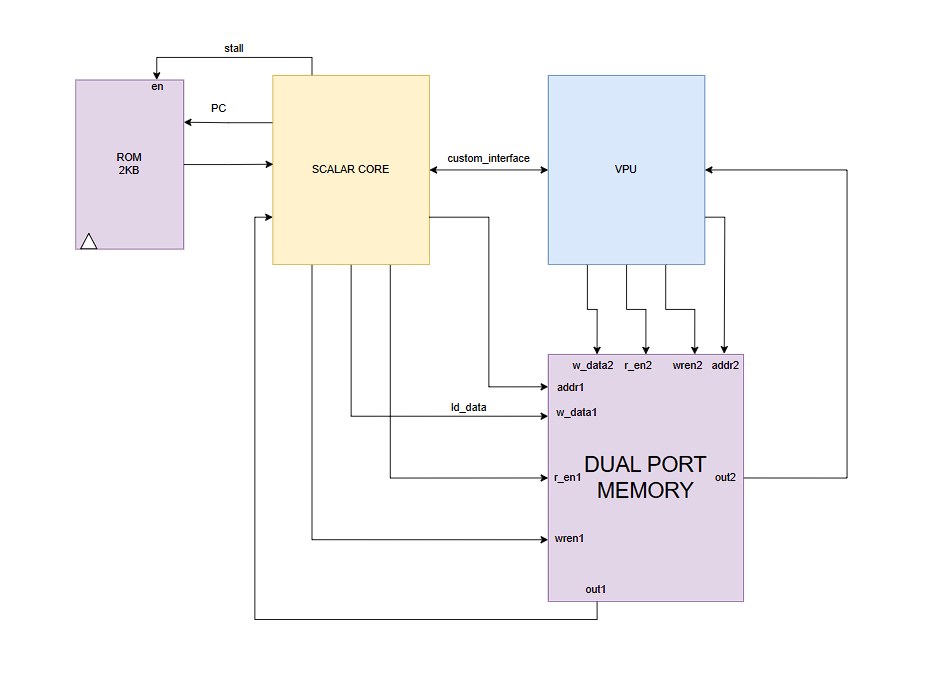
\includegraphics[width=\textwidth]{../image/harvard_architecture.png}
  \caption{Harvard memory architecture: IMEM connected to the IF stage (read-only),
           DMEM with dual scalar/VLSU ports connected to the MEM stage and vector LSU.}
  \label{fig:harvard_arch}
\end{figure}

\subsection{Instruction Memory (IMEM)}

The instruction memory is a synchronous single-port read-only memory with the
parameters shown in Table~\ref{tab:imem-spec}.

\begin{table}[H]
  \centering
  \caption{Instruction memory specification}
  \label{tab:imem-spec}
  \begin{tabular}{@{}ll@{}}
    \toprule
    \textbf{Parameter} & \textbf{Value} \\
    \midrule
    Base address          & \texttt{0x00000000} \\
    Size                  & 8~KB (2048 $\times$ 32-bit words) \\
    Access width          & 32 bits \\
    Latency               & 1 cycle (registered output) \\
    Contents              & \texttt{.text} and \texttt{.rodata} sections only \\
    Initialisation        & \texttt{\$readmemh} from \texttt{imem.hex} at simulation \\
    Write access          & None (read-only in hardware) \\
    \bottomrule
  \end{tabular}
\end{table}

The \texttt{imem.hex} file is generated from the compiled firmware ELF by the
\texttt{elf2hex\_lines.py} script, which converts the raw binary into one 32-bit
word per line in hexadecimal format. The linker script (\texttt{sw/link.ld}) places
\texttt{.text} at \texttt{0x00000000} and limits the total code size to 8~KB.

\subsection{Data Memory (DMEM)}

The data memory is a synchronous dual-port block RAM with the parameters shown in
Table~\ref{tab:dmem-spec}. Port~A services scalar load/store requests from the scalar
pipeline's MEM stage. Port~B services vector load/store requests from the VLSU.
Both ports can operate simultaneously, enabling the scalar and vector pipelines to
access memory in the same clock cycle without mutual stalling.

\begin{table}[H]
  \centering
  \caption{Data memory specification}
  \label{tab:dmem-spec}
  \begin{tabular}{@{}lll@{}}
    \toprule
    \textbf{Parameter} & \textbf{Port A (Scalar)} & \textbf{Port B (VLSU)} \\
    \midrule
    Base address   & \texttt{0x00000000} & \texttt{0x00000000} \\
    Size           & \multicolumn{2}{c}{64~KB (16384 $\times$ 32-bit words)} \\
    Access width   & 32 bits (byte-enable) & 32 bits (byte-enable) \\
    Latency        & 1 cycle              & 1 cycle \\
    Write support  & Yes                  & Yes (vector stores) \\
    Byte enable    & 4-bit mask           & 4-bit mask \\
    \bottomrule
  \end{tabular}
\end{table}

The VLSU uses \texttt{addr[15:2]} as the word index into the 64KB DMEM, consistent
with word-addressed access. Byte-enable signals allow sub-word writes for 8-bit and
16-bit vector element widths.

\subsection{Address Decode}

The scalar pipeline's LSU decodes memory addresses as follows:

\begin{itemize}
  \item \texttt{addr[31:8] == 24'h000000}: DMEM access (routed to Port~A of DMEM).
  \item \texttt{addr[31:8] == 24'hFF0000}: UART MMIO access (routed to UART TL-UL slave).
  \item All other addresses: undefined behaviour (no response, reads return zero).
\end{itemize}

The VLSU always accesses DMEM via Port~B regardless of the address, since vector
data is guaranteed by the firmware to reside in the DMEM range.

\section{UART Interface Specification}
\label{sec:uart-spec}

\subsection{Physical Framing}

The UART interface uses the 8-N-1 framing format: one start bit (logic 0), eight data
bits (LSB first), no parity bit, and one stop bit (logic 1). The baud rate is
configurable via RTL parameters but defaults to 115200~baud for production firmware.

At 115200~baud, the bit period is $1/115200 \approx 8.68~\mu$s. The UART baud clock
is derived by dividing the system clock by a baud divisor:
\begin{equation}
  \text{baud\_div} = \left\lfloor \frac{f_\text{clk}}{\text{baud\_rate}} \right\rfloor
  \label{eq:baud-div}
\end{equation}
For the simulation default of $f_\text{clk} = 14.7456~\text{MHz}$, baud\_div=128,
giving 128 clock cycles per bit. For the FPGA default of $f_\text{clk} = 50~\text{MHz}$,
baud\_div=434.

\subsection{MMIO Register Map}

The UART is mapped as a TileLink Uncached Lightweight (\gls{tlu}) slave at base address
\texttt{0xFF000000}. Table~\ref{tab:uart-regs} shows the register map.

\begin{table}[H]
  \centering
  \caption{UART MMIO register map}
  \label{tab:uart-regs}
  \begin{tabular}{@{}llll@{}}
    \toprule
    \textbf{Offset} & \textbf{Register} & \textbf{Access} & \textbf{Description} \\
    \midrule
    \texttt{+0x00} & CTRL   & RW & Control register (reserved for future use) \\
    \texttt{+0x04} & STAT   & RO & Status register \\
    \texttt{+0x08} & TXDAT  & WO & Transmit data register \\
    \texttt{+0x0C} & RXDAT  & RO & Receive data register \\
    \bottomrule
  \end{tabular}
\end{table}

\subsubsection{STAT Register (offset +0x04)}

\begin{table}[H]
  \centering
  \caption{UART STAT register bit assignments}
  \label{tab:uart-stat}
  \begin{tabular}{@{}cll@{}}
    \toprule
    \textbf{Bit} & \textbf{Field} & \textbf{Description} \\
    \midrule
    \texttt{[0]} & \texttt{tx\_ready} & 1 = TX shift register is empty, ready for new byte \\
    \texttt{[1]} & \texttt{rx\_valid} & 1 = RX FIFO contains at least one byte \\
    \texttt{[31:2]} & ---            & Reserved, read as zero \\
    \bottomrule
  \end{tabular}
\end{table}

\subsubsection{TXDAT Register (offset +0x08)}

Writing a byte to this register loads it into the transmit shift register. Writes are
ignored if \texttt{tx\_ready} is 0. Firmware must poll \texttt{tx\_ready} in the STAT
register before each write to avoid dropping characters.

\subsubsection{RXDAT Register (offset +0x0C)}

Reading this register returns the oldest byte in the receive FIFO in bits [7:0].
Bits [31:8] read as zero. If \texttt{rx\_valid} is 0, the read returns an undefined
value. Firmware must poll \texttt{rx\_valid} in the STAT register before each read.

\subsection{Firmware Programming Model}

A typical firmware receive-byte function polls the STAT register until \texttt{rx\_valid}
is set, then reads RXDAT:

\begin{lstlisting}[language=RISCV, caption={UART receive byte (polling)}]
# a0 = UART base address (0xFF000000)
# Returns received byte in a0
uart_getchar:
    li   t0, 0xFF000000   # UART base
.wait_rx:
    lw   t1, 4(t0)        # read STAT
    andi t1, t1, 2        # test rx_valid bit
    beqz t1, .wait_rx     # spin until byte available
    lw   a0, 12(t0)       # read RXDAT
    andi a0, a0, 0xFF     # mask to 8 bits
    ret
\end{lstlisting}

\begin{lstlisting}[language=RISCV, caption={UART transmit byte (polling)}]
# a0 = byte to transmit
# Uses t0--t1 as temporaries
uart_putchar:
    li   t0, 0xFF000000   # UART base
.wait_tx:
    lw   t1, 4(t0)        # read STAT
    andi t1, t1, 1        # test tx_ready bit
    beqz t1, .wait_tx     # spin until TX ready
    sw   a0, 8(t0)        # write TXDAT
    ret
\end{lstlisting}

\subsection{Timing Constraints}

The UART's TL-UL slave interface is registered: the channel-D response to a channel-A
request is registered at the output, introducing a one-cycle read latency. This matches
the one-cycle latency of the DMEM, ensuring that the scalar pipeline's load path has
the same timing whether accessing DMEM or the UART.

For synthesis, the UART datapath must meet setup timing at the target clock frequency.
The baud divisor counter is a simple 16-bit counter; its path from counter register
to the baud-clock enable is not on the critical path. The TL-UL address comparator
(checking \texttt{addr[31:8] == 24'hFF0000}) adds one level of logic to the address
decode path, which is accounted for in the FPGA timing analysis.

\section{Performance Requirements}
\label{sec:perf-requirements}

\subsection{Target Clock Frequency}

The design shall achieve a minimum $F_\text{max}$ of 50~MHz on the Intel Cyclone~V
(5CSXFC6D6F31C8) device used on the DE10-Standard board \cite{de10standard}. This
target is chosen to enable real-time processing of a 640$\times$480 video frame
at approximately 2~frames per second with the single-lane architecture, providing
a meaningful demonstration of the vector processing capability.

At 50~MHz with VLEN=128, SEW=8, and LMUL=1 (16 elements per cycle), the VLSU achieves
a data throughput of:
\begin{equation}
  \text{Throughput}_\text{load} = 50 \times 10^6 \text{ Hz} \times \frac{4~\text{bytes}}{\text{cycle}} = 200~\text{MB/s}
  \label{eq:load-throughput}
\end{equation}
for unit-stride loads (one 32-bit word per cycle from DMEM).

For arithmetic throughput at SEW=8, the single-lane processes 4 elements per 32-bit
lane per cycle when the cycle counter advances, giving 4~Gops/s at 1~GHz or 200~Mops/s
at 50~MHz. The BT.601 grayscale benchmark requires $3 \times 16384 = 49152$ multiply
operations and 16384 additions for the luminance channel of a 128$\times$128 image;
at 200~Mops/s this completes in approximately 0.33~ms.

\subsection{Area Budget}

The target area budget for FPGA prototyping is 12000~\glspl{alm} on the Cyclone~V
device. This leaves sufficient resources for debugging logic, block RAM, and any
future additions. The measured area after synthesis and place-and-route is 10438~ALMs,
confirming that the implementation meets this budget with approximately 13\% headroom.

For a future ASIC implementation in a 28nm or 22nm technology node, an informal
estimate based on the ALM count and typical ALM-to-gate ratios suggests a target
of 50000--100000 standard-cell gate equivalents for the core logic, excluding
memory macros.

\subsection{Power Estimation}

Quantitative power estimates for the FPGA prototype are not the primary deliverable
of this thesis; the FPGA fabric's configurable routing introduces significant static
power overhead that is not representative of an ASIC implementation. However, the
design incorporates clock-gating enable signals (\texttt{vrf\_wren}, \texttt{*\_en})
on the vector register file and LSU data-path registers so that power estimation tools
in a future ASIC flow can infer clock gating cells at these control points, meeting
the ASIC design rule requiring explicit enable signals on all high-fan-out registers.
